%!TeX root=../princesstop.tex
\chapter{Anne}

\begin{figure}[t!]
\centering
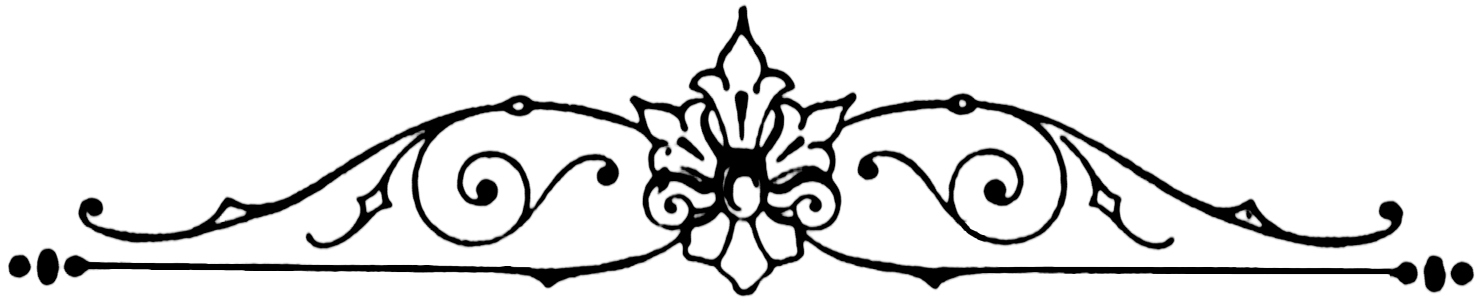
\includegraphics[width=\linewidth]{filigree}
\end{figure}

\lettrine[lines=5]{N}{ever} had such joy reigned in the nursery of the Large Family. Never had they dreamed of such delights as resulted from an intimate acquaintance with the little-girl-who-was-not-a-beggar. The mere fact of her sufferings and adventures made her a priceless possession. Everybody wanted to be told over and over again the things which had happened to her. When one was sitting by a warm fire in a big, glowing room, it was quite delightful to hear how cold it could be in an attic. It must be admitted that the attic was rather delighted in, and that its coldness and bareness quite sank into insignificance when Melchisedec was remembered, and one heard about the sparrows and things one could see if one climbed on the table and stuck one's head and shoulders out of the skylight.

Of course the thing loved best was the story of the banquet and the dream which was true. Sara told it for the first time the day after she had been found. Several members of the Large Family came to take tea with her, and as they sat or curled up on the hearth-rug she told the story in her own way, and the Indian gentleman listened and watched her. When she had finished she looked up at him and put her hand on his knee.

<That is my part,> she said. <Now won't you tell your part of it, Uncle Tom?> He had asked her to call him always <Uncle Tom.> <I don't know your part yet, and it must be beautiful.>

So he told them how, when he sat alone, ill and dull and irritable, Ram Dass had tried to distract him by describing the passers by, and there was one child who passed oftener than any one else; he had begun to be interested in her—partly perhaps because he was thinking a great deal of a little girl, and partly because Ram Dass had been able to relate the incident of his visit to the attic in chase of the monkey. He had described its cheerless look, and the bearing of the child, who seemed as if she was not of the class of those who were treated as drudges and servants. Bit by bit, Ram Dass had made discoveries concerning the wretchedness of her life. He had found out how easy a matter it was to climb across the few yards of roof to the skylight, and this fact had been the beginning of all that followed.

<Sahib,> he had said one day, <I could cross the slates and make the child a fire when she is out on some errand. When she returned, wet and cold, to find it blazing, she would think a magician had done it.>

The idea had been so fanciful that Mr Carrisford's sad face had lighted with a smile, and Ram Dass had been so filled with rapture that he had enlarged upon it and explained to his master how simple it would be to accomplish numbers of other things. He had shown a childlike pleasure and invention, and the preparations for the carrying out of the plan had filled many a day with interest which would otherwise have dragged wearily. On the night of the frustrated banquet Ram Dass had kept watch, all his packages being in readiness in the attic which was his own; and the person who was to help him had waited with him, as interested as himself in the odd adventure. Ram Dass had been lying flat upon the slates, looking in at the skylight, when the banquet had come to its disastrous conclusion; he had been sure of the profoundness of Sara's wearied sleep; and then, with a dark lantern, he had crept into the room, while his companion remained outside and handed the things to him. When Sara had stirred ever so faintly, Ram Dass had closed the lantern-slide and lain flat upon the floor. These and many other exciting things the children found out by asking a thousand questions.

<I am so glad,> Sara said. <I am so \textsc{glad} it was you who were my friend!>

There never were such friends as these two became. Somehow, they seemed to suit each other in a wonderful way. The Indian gentleman had never had a companion he liked quite as much as he liked Sara. In a month's time he was, as Mr Carmichael had prophesied he would be, a new man. He was always amused and interested, and he began to find an actual pleasure in the possession of the wealth he had imagined that he loathed the burden of. There were so many charming things to plan for Sara. There was a little joke between them that he was a magician, and it was one of his pleasures to invent things to surprise her. She found beautiful new flowers growing in her room, whimsical little gifts tucked under pillows, and once, as they sat together in the evening, they heard the scratch of a heavy paw on the door, and when Sara went to find out what it was, there stood a great dog—a splendid Russian boarhound—with a grand silver and gold collar bearing an inscription. <I am Boris,> it read; <I serve the Princess Sara.>

There was nothing the Indian gentleman loved more than the recollection of the little princess in rags and tatters. The afternoons in which the Large Family, or Ermengarde and Lottie, gathered to rejoice together were very delightful. But the hours when Sara and the Indian gentleman sat alone and read or talked had a special charm of their own. During their passing many interesting things occurred.

One evening, Mr Carrisford, looking up from his book, noticed that his companion had not stirred for some time, but sat gazing into the fire.

<What are you <supposing,> Sara?> he asked.

Sara looked up, with a bright colour on her cheek.

<I \textsc{was} supposing,> she said; <I was remembering that hungry day, and a child I saw.>

<But there were a great many hungry days,> said the Indian gentleman, with rather a sad tone in his voice. <Which hungry day was it?>

<I forgot you didn't know,> said Sara. <It was the day the dream came true.>

Then she told him the story of the bun shop, and the fourpence she picked up out of the sloppy mud, and the child who was hungrier than herself. She told it quite simply, and in as few words as possible; but somehow the Indian gentleman found it necessary to shade his eyes with his hand and look down at the carpet.

<And I was supposing a kind of plan,> she said, when she had finished. <I was thinking I should like to do something.>

<What was it?> said Mr Carrisford, in a low tone. <You may do anything you like to do, princess.>

<I was wondering,> rather hesitated Sara—<you know, you say I have so much money—I was wondering if I could go to see the bun-woman, and tell her that if, when hungry children—particularly on those dreadful days—come and sit on the steps, or look in at the window, she would just call them in and give them something to eat, she might send the bills to me. Could I do that?>

<You shall do it tomorrow morning,> said the Indian gentleman.

<Thank you,> said Sara. <You see, I know what it is to be hungry, and it is very hard when one cannot even \textsc{pretend} it away.>

<Yes, yes, my dear,> said the Indian gentleman. <Yes, yes, it must be. Try to forget it. Come and sit on this footstool near my knee, and only remember you are a princess.>

<Yes,> said Sara, smiling; <and I can give buns and bread to the populace.> And she went and sat on the stool, and the Indian gentleman (he used to like her to call him that, too, sometimes) drew her small dark head down on his knee and stroked her hair.

The next morning, Miss Minchin, in looking out of her window, saw the things she perhaps least enjoyed seeing. The Indian gentleman's carriage, with its tall horses, drew up before the door of the next house, and its owner and a little figure, warm with soft, rich furs, descended the steps to get into it. The little figure was a familiar one, and reminded Miss Minchin of days in the past. It was followed by another as familiar—the sight of which she found very irritating. It was Becky, who, in the character of delighted attendant, always accompanied her young mistress to her carriage, carrying wraps and belongings. Already Becky had a pink, round face.

A little later the carriage drew up before the door of the baker's shop, and its occupants got out, oddly enough, just as the bun-woman was putting a tray of smoking-hot buns into the window.

When Sara entered the shop the woman turned and looked at her, and, leaving the buns, came and stood behind the counter. For a moment she looked at Sara very hard indeed, and then her good-natured face lighted up.

<I'm sure that I remember you, miss,> she said. <And yet\longdash>

<Yes,> said Sara; <once you gave me six buns for fourpence, and\longdash>

<And you gave five of 'em to a beggar child,> the woman broke in on her. <I've always remembered it. I couldn't make it out at first.> She turned round to the Indian gentleman and spoke her next words to him. <I beg your pardon, sir, but there's not many young people that notices a hungry face in that way; and I've thought of it many a time. Excuse the liberty, miss,>—to Sara—<but you look rosier and—well, better than you did that—that\longdash>

<I am better, thank you,> said Sara. <And—I am much happier—and I have come to ask you to do something for me.>

<Me, miss!> exclaimed the bun-woman, smiling cheerfully. <Why, bless you! Yes, miss. What can I do?>

And then Sara, leaning on the counter, made her little proposal concerning the dreadful days and the hungry waifs and the buns.

The woman watched her, and listened with an astonished face.

<Why, bless me!> she said again when she had heard it all; <it'll be a pleasure to me to do it. I am a working-woman myself and cannot afford to do much on my own account, and there's sights of trouble on every side; but, if you'll excuse me, I'm bound to say I've given away many a bit of bread since that wet afternoon, just along o' thinking of you—an' how wet an' cold you was, an' how hungry you looked; an' yet you gave away your hot buns as if you was a princess.>

The Indian gentleman smiled involuntarily at this, and Sara smiled a little, too, remembering what she had said to herself when she put the buns down on the ravenous child's ragged lap.

<She looked so hungry,> she said. <She was even hungrier than I was.>

<She was starving,> said the woman. <Many's the time she's told me of it since—how she sat there in the wet, and felt as if a wolf was a-tearing at her poor young insides.>

<Oh, have you seen her since then?> exclaimed Sara. <Do you know where she is?>

<Yes, I do,> answered the woman, smiling more good-naturedly than ever. <Why, she's in that there back room, miss, an' has been for a month; an' a decent, well-meanin' girl she's goin' to turn out, an' such a help to me in the shop an' in the kitchen as you'd scarce believe, knowin' how she's lived.>

She stepped to the door of the little back parlour and spoke; and the next minute a girl came out and followed her behind the counter. And actually it was the beggar-child, clean and neatly clothed, and looking as if she had not been hungry for a long time. She looked shy, but she had a nice face, now that she was no longer a savage, and the wild look had gone from her eyes. She knew Sara in an instant, and stood and looked at her as if she could never look enough.

<You see,> said the woman, <I told her to come when she was hungry, and when she'd come I'd give her odd jobs to do; an' I found she was willing, and somehow I got to like her; and the end of it was, I've given her a place an' a home, and she helps me, an' behaves well, an' is as thankful as a girl can be. Her name's Anne. She has no other.>

The children stood and looked at each other for a few minutes; and then Sara took her hand out of her muff and held it out across the counter, and Anne took it, and they looked straight into each other's eyes.

<I am so glad,> Sara said. <And I have just thought of something. Perhaps Mrs Brown will let you be the one to give the buns and bread to the children. Perhaps you would like to do it because you know what it is to be hungry, too.>

<Yes, miss,> said the girl.

And, somehow, Sara felt as if she understood her, though she said so little, and only stood still and looked and looked after her as she went out of the shop with the Indian gentleman, and they got into the carriage and drove away.

\vfill
\begin{center}
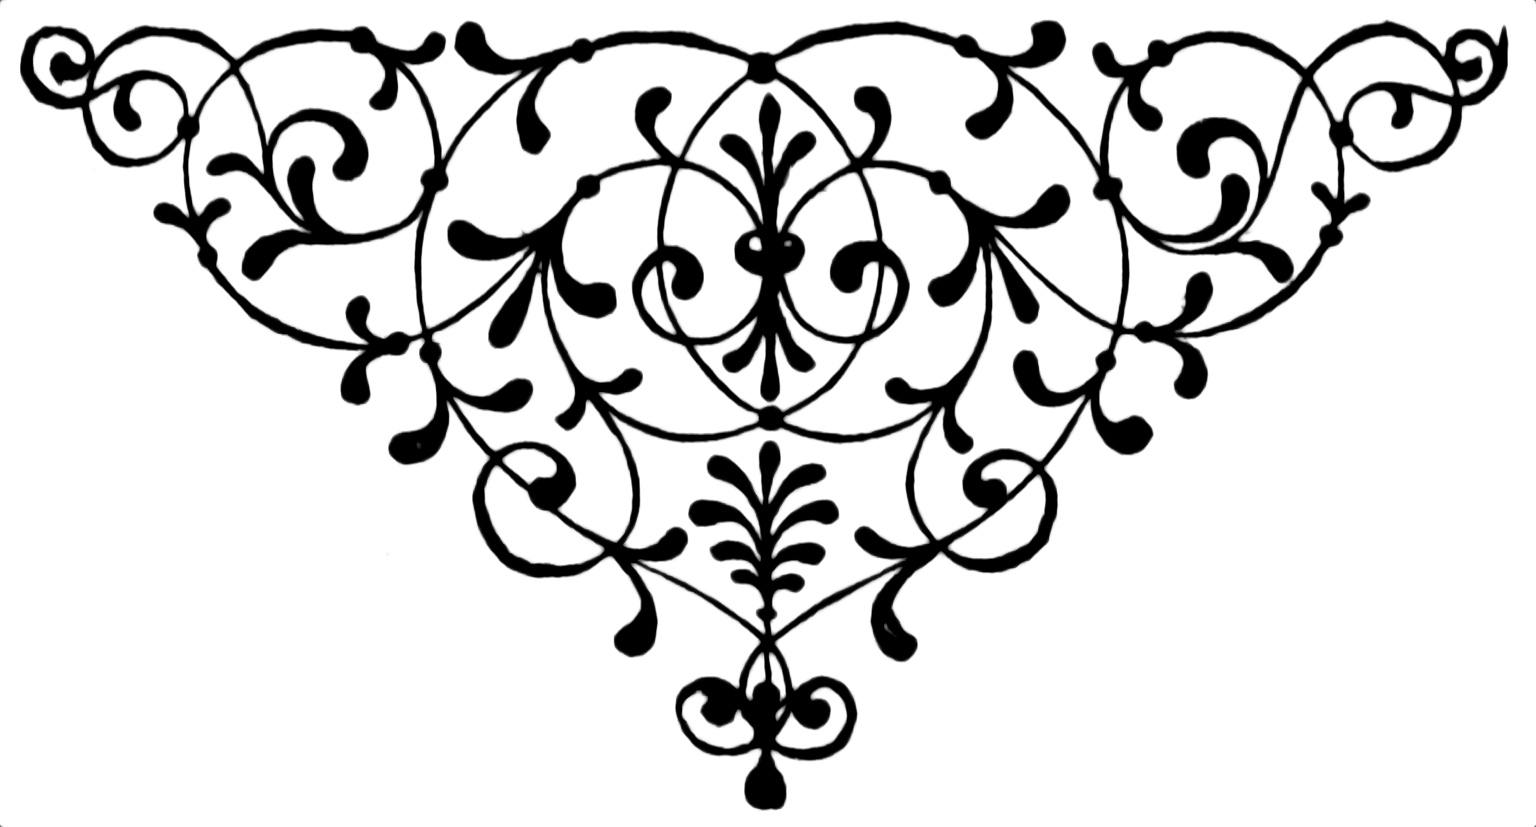
\includegraphics[width=.8\linewidth]{theend}
\end{center}